\task{Изображения на плоскости}

\begin{flushright} \itshape
	Алгоритм Тарского, не так ли?
\end{flushright}

\ms В данной задаче нас будет интересовать возможность представить множество точек на плоскости как множество решений какого-либо уравнения или неравенства. Например, уравнение $x - y = 0$ задает прямую с углом наклона $45^\circ$, а неравенство $min (x,y) \geq 0$ — первую координатную четверть.

\ms При составлении неравенств и уравнений вам разрешено пользоваться арифметическими действиями — сложением, умножением, вычитанием, делением; функцией модуля — $|\ldots|$, а также $\max$ и $\min$ — взятием наибольшего и наименьшего значений из конечного набора чисел.

\begin{enumerate}
\item Докажите, что

\subitem (а) $A \cdot B > 0$ тогда и только тогда, когда числа $A$ и $B$ одного знака;
\subitem (б) $\min (x,y) = \frac{1}{2} \Bigl( x + y - |x - y| \Bigr)$;
\subitem (в) Даны числа $a_1 < a_2 < \ldots < a_n$. Докажите, что если $a_k < x < a_{k+1}$, то знак выражения

\vspace{-0.3cm}
$$(x-a_1)\cdot (x-a_2)\cdot \ldots \cdot (x-a_n)$$

\vspace{-0.15cm}
совпадает со знаком выражения $(-1)^n \cdot (-1)^k$.

\item Изобразите множество точек $(x,y)$ на плоскости, удовлетворяющих неравенству

\vspace{-0.3cm}
$$\max(|x|, |y|)\,\geq\,1.$$

\item Множеством решений какого неравенства является (а) горизон-\linebreak тальная полоса на плоскости (б) наклонная полоса на плоскости\linebreak (смотреть рисунок)?

\centerline{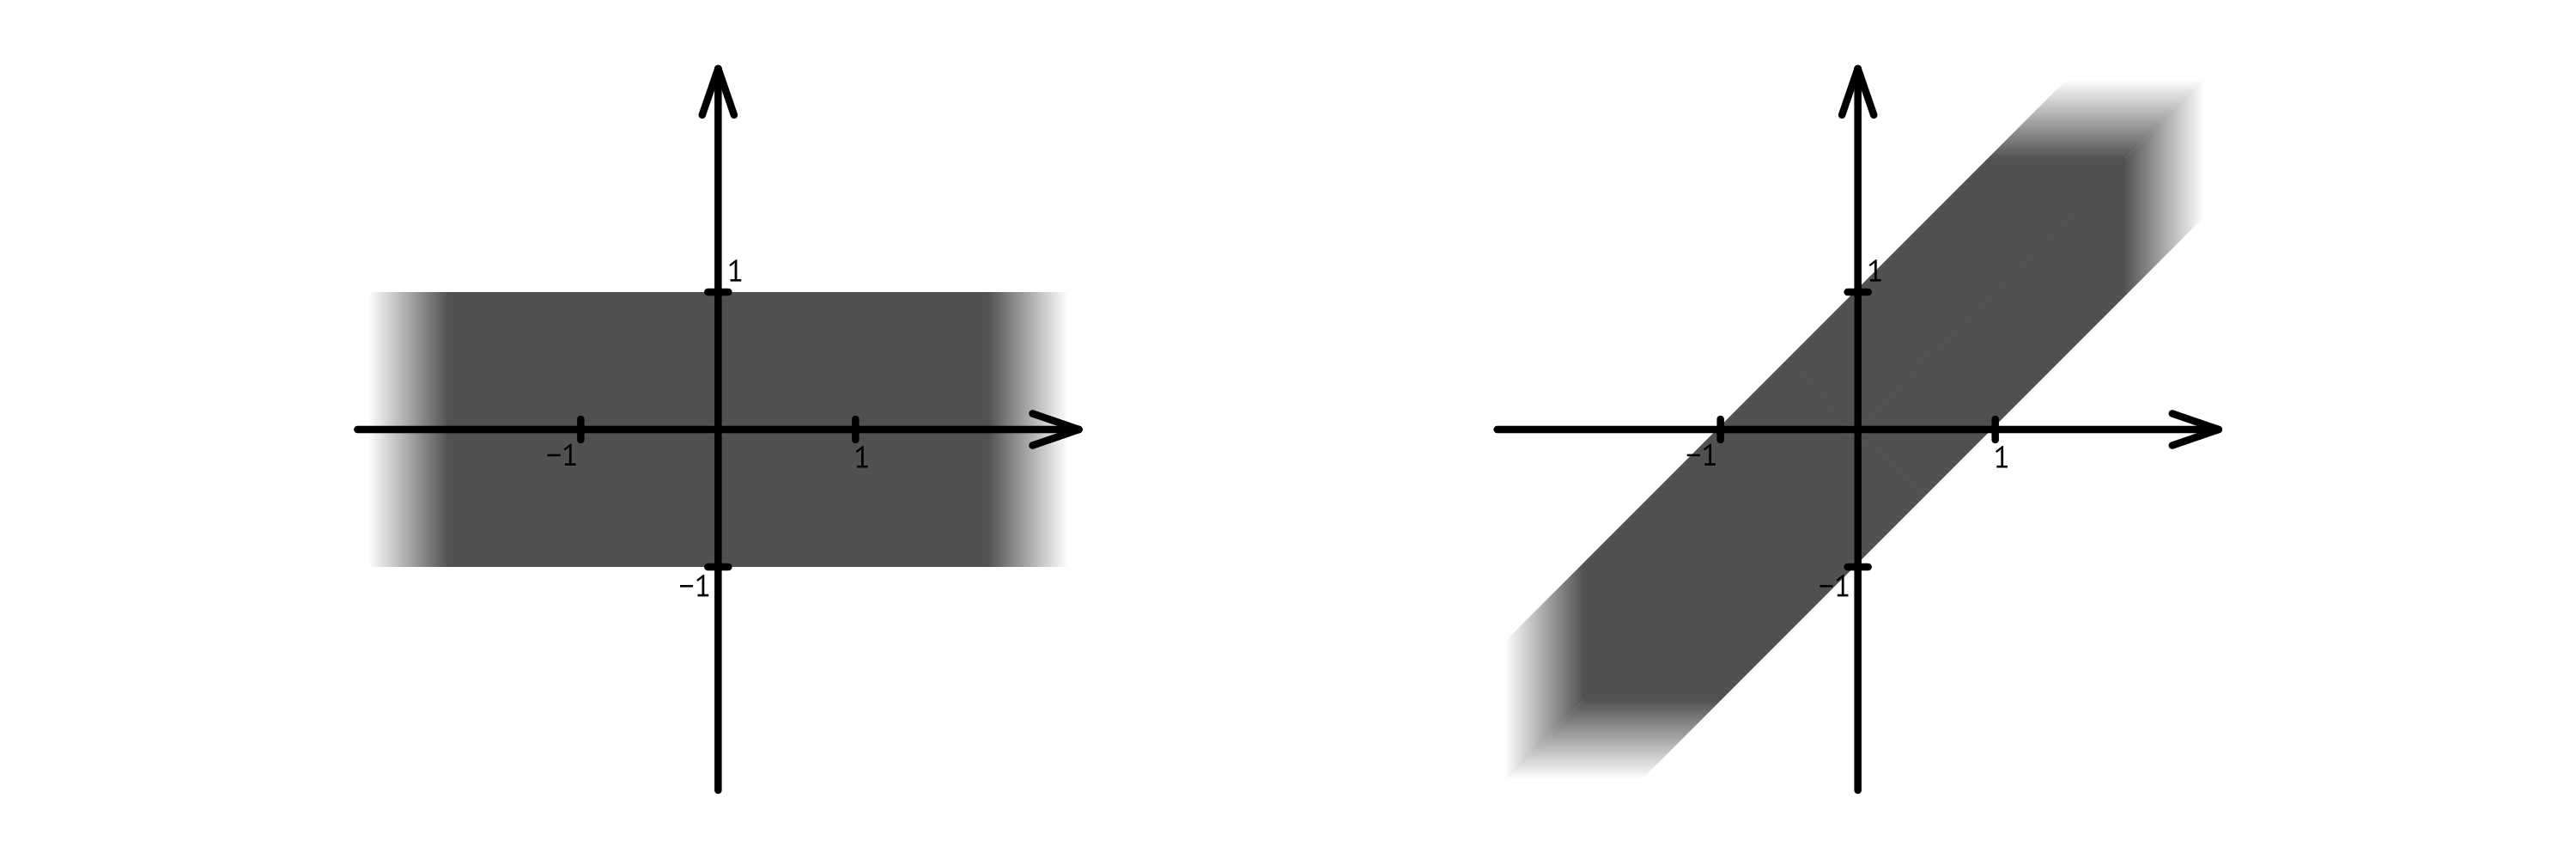
\includegraphics[width=13.75cm]{stats/2018/graph/1}}

\item Множеством решений какого неравенства является (а) «крестик» на плоскости (б) фигура, полученная из круга и полуплоскости (смотреть рисунок)?

\centerline{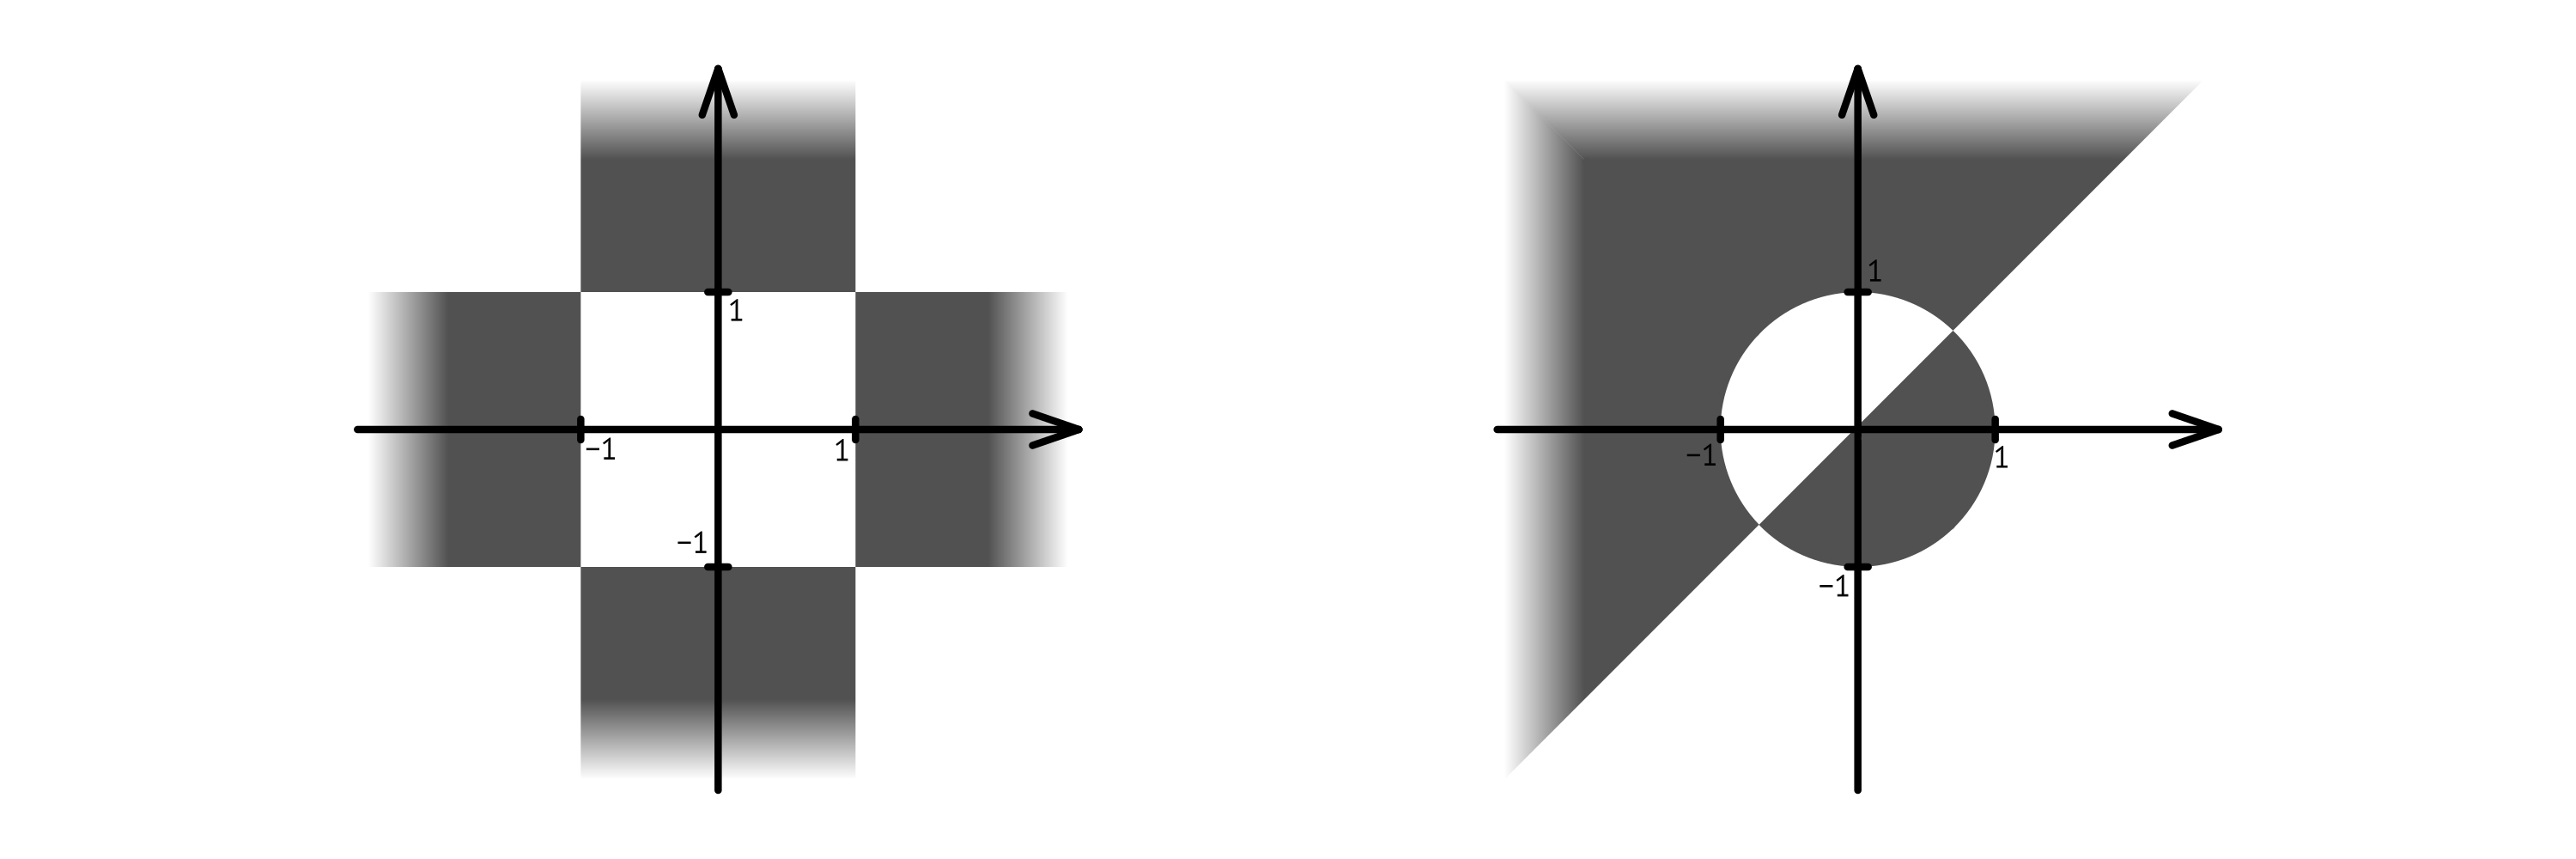
\includegraphics[width=13.75cm]{stats/2018/graph/2}}

\item Множеством решений какого неравенства является фигура (смотреть рисунок), полученная из трех кругов радиуса $1.5$ с центрами в точках $(1,\,-1)$, $(-1,\,-1)$, $(0,\,0.5)$?

\centerline{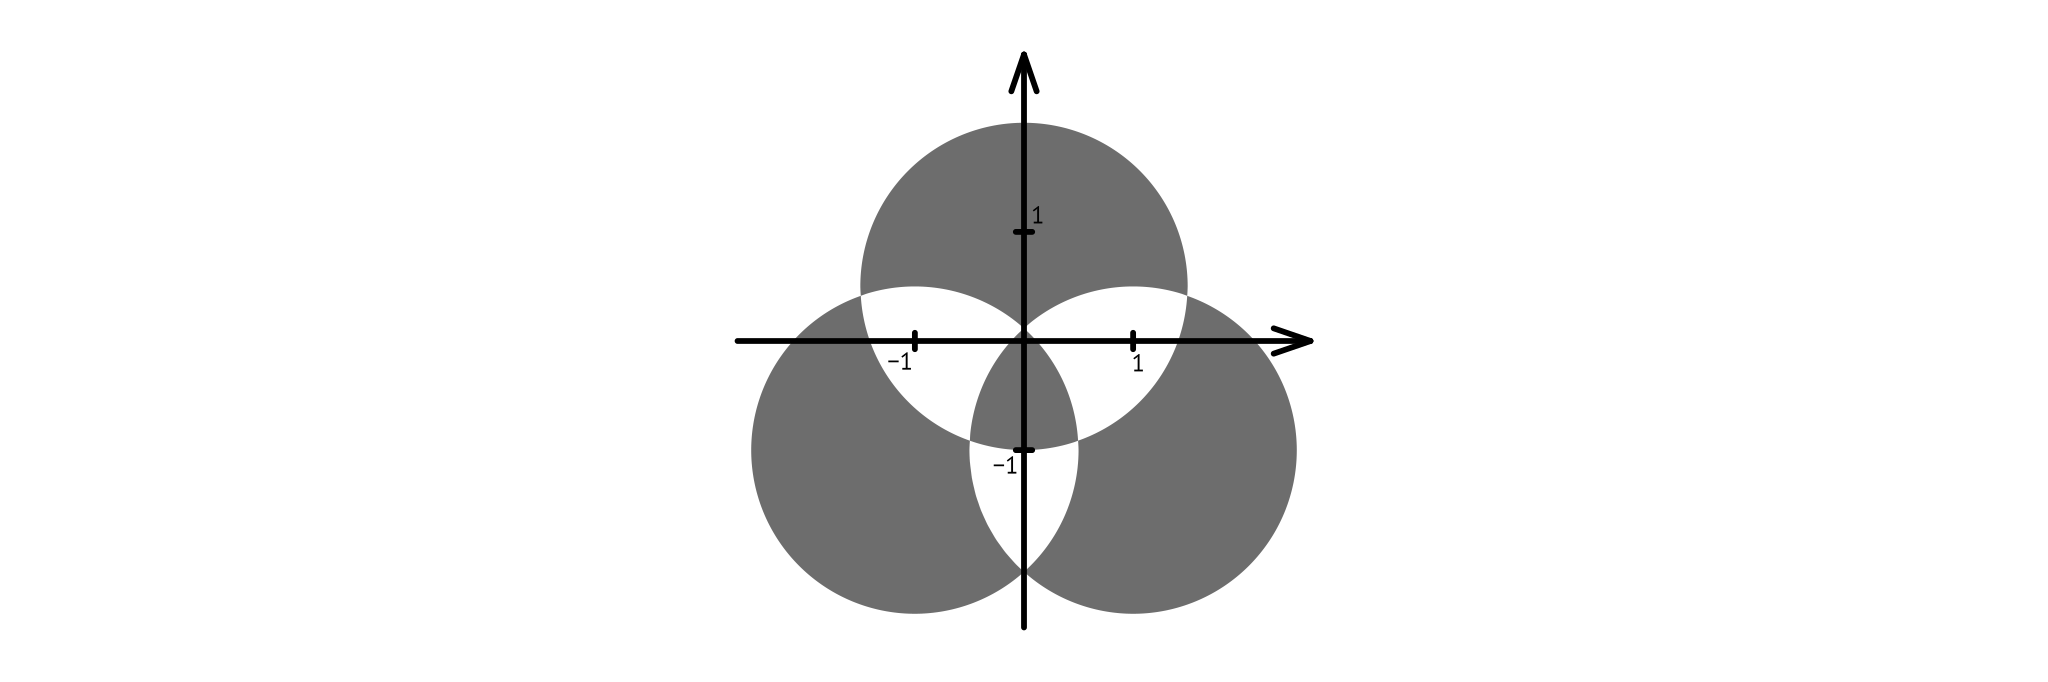
\includegraphics[width=13.75cm]{stats/2018/graph/3}}

\item Множеством решений какого уравнения является (а) фигура из трех окружностей (б) фигура из трех лучей (смотреть рисунок)?

\centerline{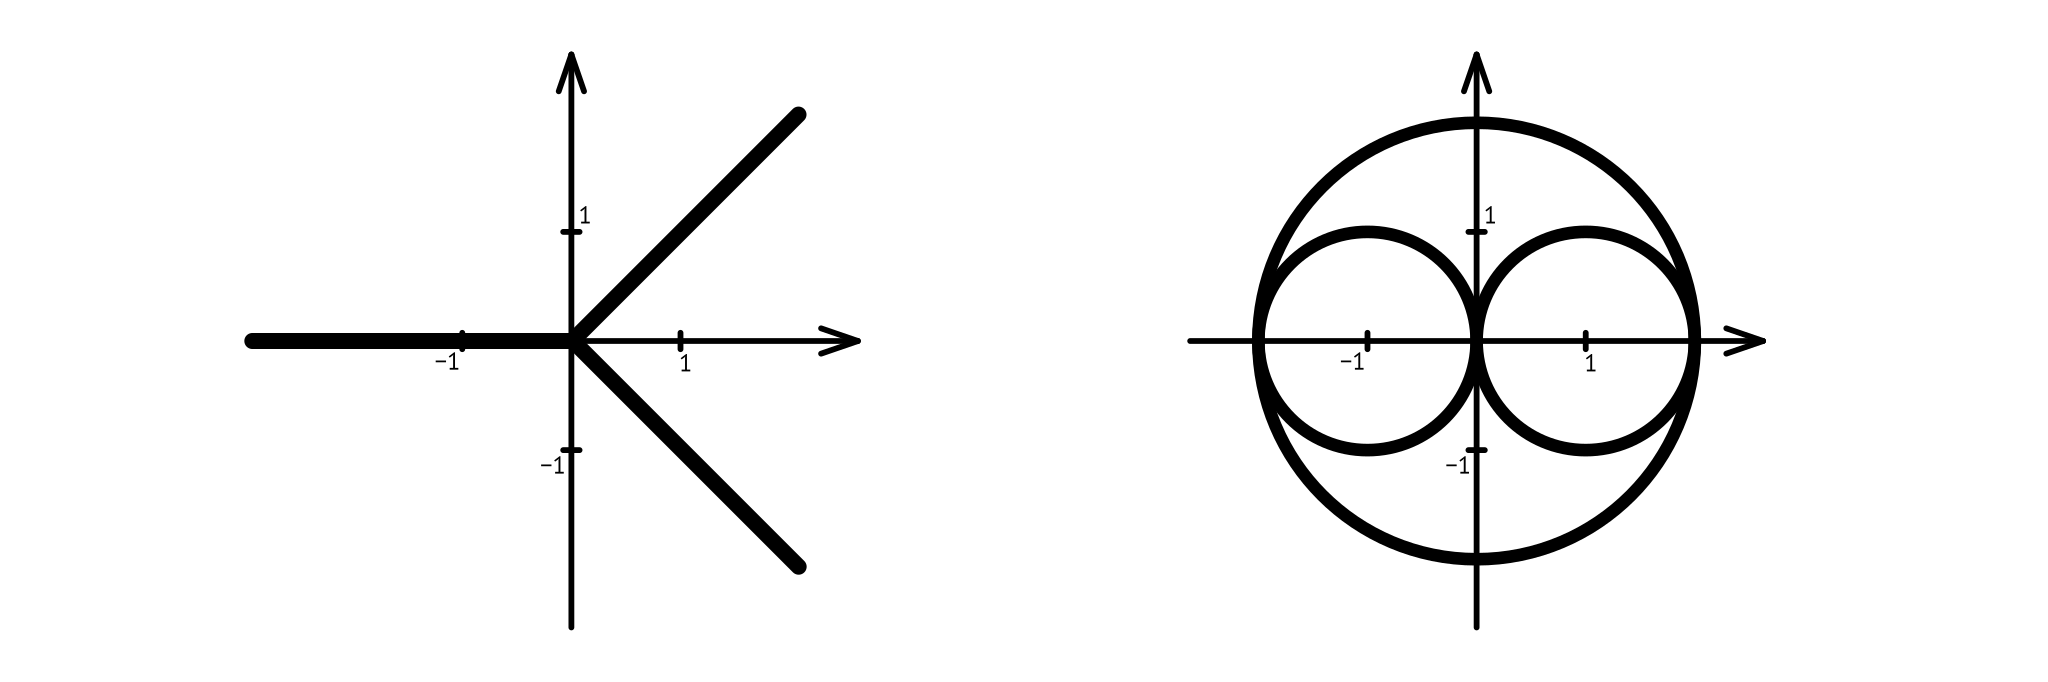
\includegraphics[width=13.75cm]{stats/2018/graph/4}}

\item Пусть фигура $F_1$~— множество решений уравнения $P_1(x,y) = 0$, а $F_2$~— множество решений уравнения $P_2 (x,y) = 0$. Приведите уравнение, решения которого образуют (а) пересечение фигур $F_1$ и $F_2$ (б) объединение фигур $F_1$ и $F_2$?

\item Пусть фигура $F_1$ — множество решений неравенства $P_1(x,y) < 0$, а $F_2$ — множество решений неравенства $P_2 (x,y) < 0$. Приведите неравенства, решения которого образуют (а) пересечение фигур $F_1$ и $F_2$ (б) объединение фигур $F_1$ и $F_2$ (в) множество точек, лежащих либо в фигуре $F_1$, либо в фигуре $F_2$, но не в них обеих одновременно?

\end{enumerate}